% =============================================================================
% PART B - MODULE 34-36: MODERATION, ID VERIFICATION \& FORUM TRASH
% In Charge: Pham Kha Vy
% =============================================================================
\subsection{Module 34--36: Moderation, ID Verification \& Forum Trash}

\subsubsection{M34.01 -- View Moderation Queue (UC-34.01)}
\begin{itemize}[leftmargin=1.5em,itemsep=2pt]
  \item \textbf{Screen Name \& Route Path:} Moderation Queue -- \texttt{/admin/forum/moderation}.
  \item \textbf{Who Can Use This:} Administrator.
  \item \Needspace{6\baselineskip}\textbf{Before You Begin:} Signed in as Administrator.
\end{itemize}
\begin{figure}[H]\centering
  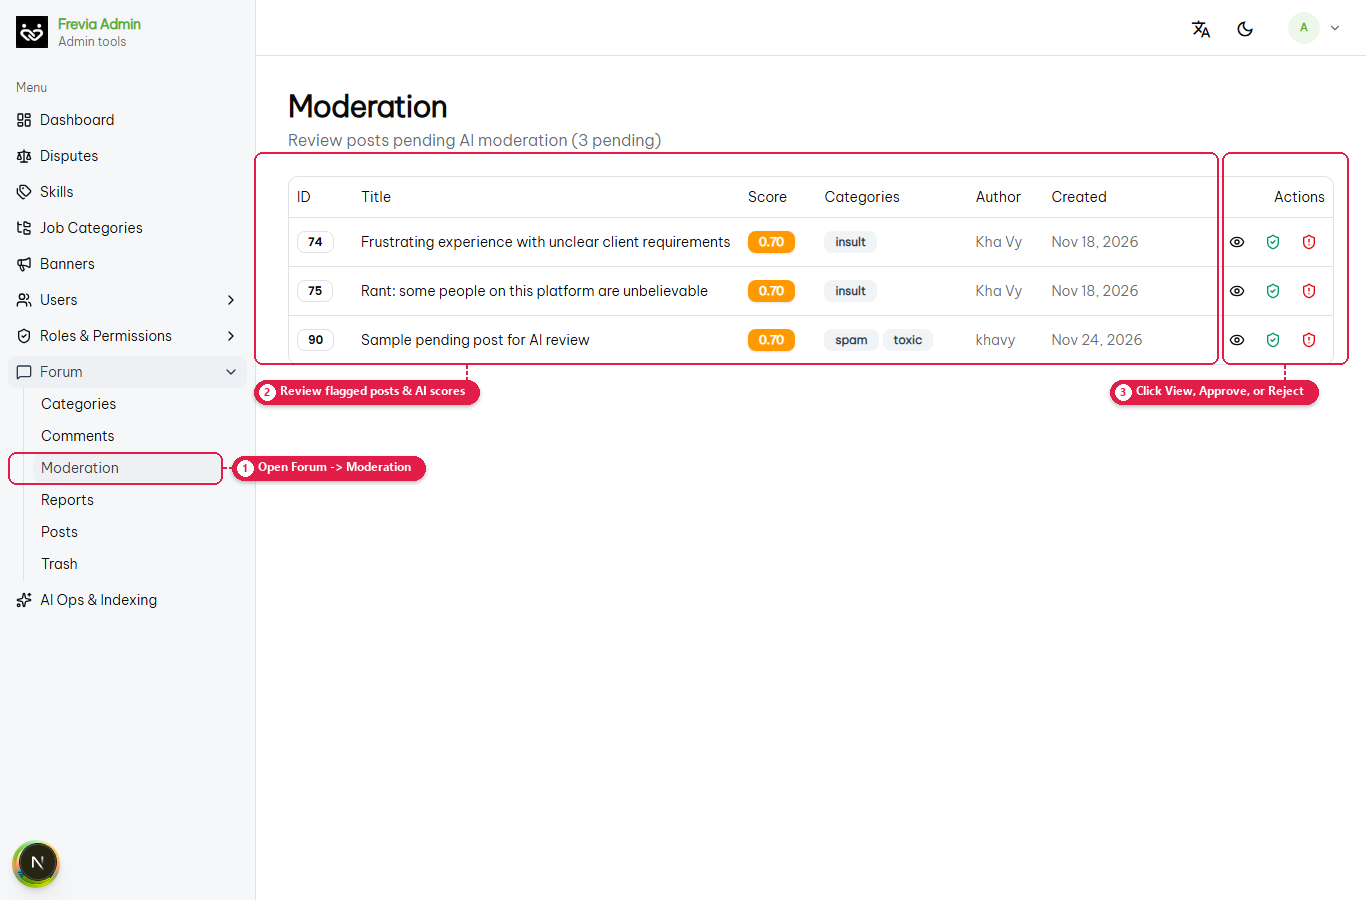
\includegraphics[width=0.90\textwidth]{images/admin/moderation/m34_01_moderation_guide.png}
  \caption{Admin Content Moderation Queue}
\end{figure}
\Needspace{6\baselineskip}\paragraph{Step-by-Step User Guide:}
\begin{enumerate}[leftmargin=1.8em,itemsep=3pt]
  \item \rbadge{1} \textbf{Search \& Filter Queue:} Filter pending or flagged posts/comments by status or keyword.
  \item \rbadge{2} \textbf{Review Risk Scores:} Inspect author, submission timestamp, and AI toxicity risk score in the table.
  \item \rbadge{3} \textbf{Open Detail / Act:} Click the Eye icon to inspect full content or approve/reject directly.
\end{enumerate}
\Needspace{6\baselineskip}\paragraph{After You Submit (Result \& Troubleshooting):}
\begin{itemize}[leftmargin=1.5em,itemsep=2pt]
  \item \textbf{What Happens Next:} All moderation queue items are listed with reporter/AI details and status.
  \item \textbf{Troubleshooting \& Common Messages:} Unauthorized users are redirected away from the admin portal.
\end{itemize}

\subsubsection{M34.02 -- View Moderation Item Detail (UC-34.02)}
\begin{itemize}[leftmargin=1.5em,itemsep=2pt]
  \item \textbf{Screen Name \& Route Path:} Moderation Detail Modal -- \texttt{/admin/forum/moderation}.
  \item \textbf{Who Can Use This:} Administrator.
  \item \Needspace{6\baselineskip}\textbf{Before You Begin:} Item exists in the moderation queue.
\end{itemize}
\begin{figure}[H]\centering
  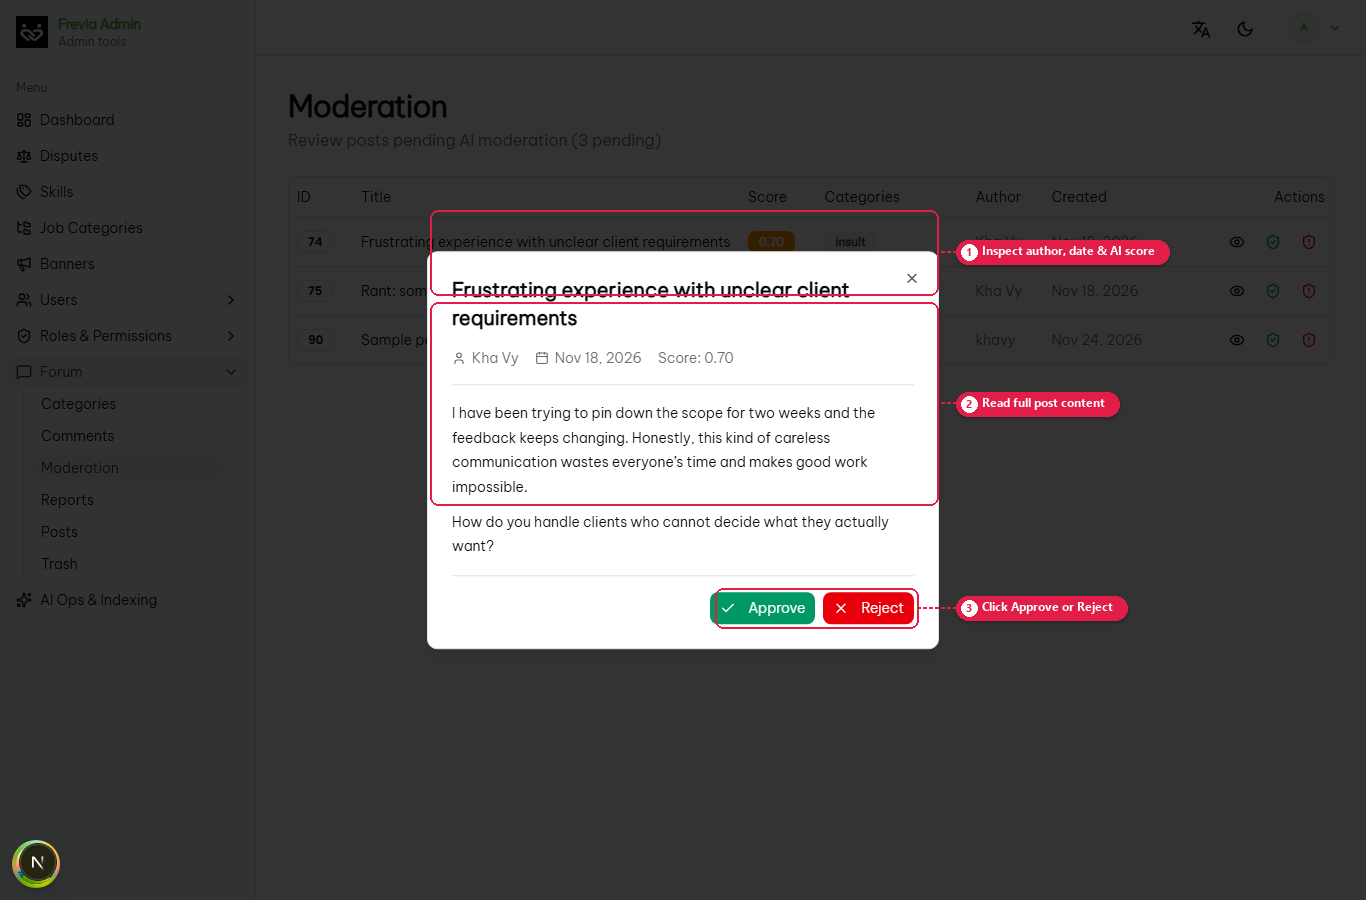
\includegraphics[width=0.90\textwidth]{images/admin/moderation/m34_02_guide.png}
  \caption{Inspecting flagged moderation item details}
\end{figure}
\Needspace{6\baselineskip}\paragraph{Step-by-Step User Guide:}
\begin{enumerate}[leftmargin=1.8em,itemsep=3pt]
  \item \rbadge{1} \textbf{Inspect Metadata:} Review the author profile, current status badge, and AI moderation score.
  \item \rbadge{2} \textbf{Read Full Content:} Read the complete post title and formatted body inside the modal.
\end{enumerate}
\Needspace{6\baselineskip}\paragraph{After You Submit (Result \& Troubleshooting):}
\begin{itemize}[leftmargin=1.5em,itemsep=2pt]
  \item \textbf{What Happens Next:} Complete item details are displayed for informed adjudication.
  \item \textbf{Troubleshooting \& Common Messages:} If the item was deleted concurrently, a not-found alert appears.
\end{itemize}

\subsubsection{M34.03 -- Resolve Moderation Item (UC-34.03)}
\begin{itemize}[leftmargin=1.5em,itemsep=2pt]
  \item \textbf{Screen Name \& Route Path:} Moderation Resolution -- \texttt{/admin/forum/moderation}.
  \item \textbf{Who Can Use This:} Administrator.
  \item \Needspace{6\baselineskip}\textbf{Before You Begin:} Moderation item is in PENDING state.
\end{itemize}
\begin{figure}[H]\centering
  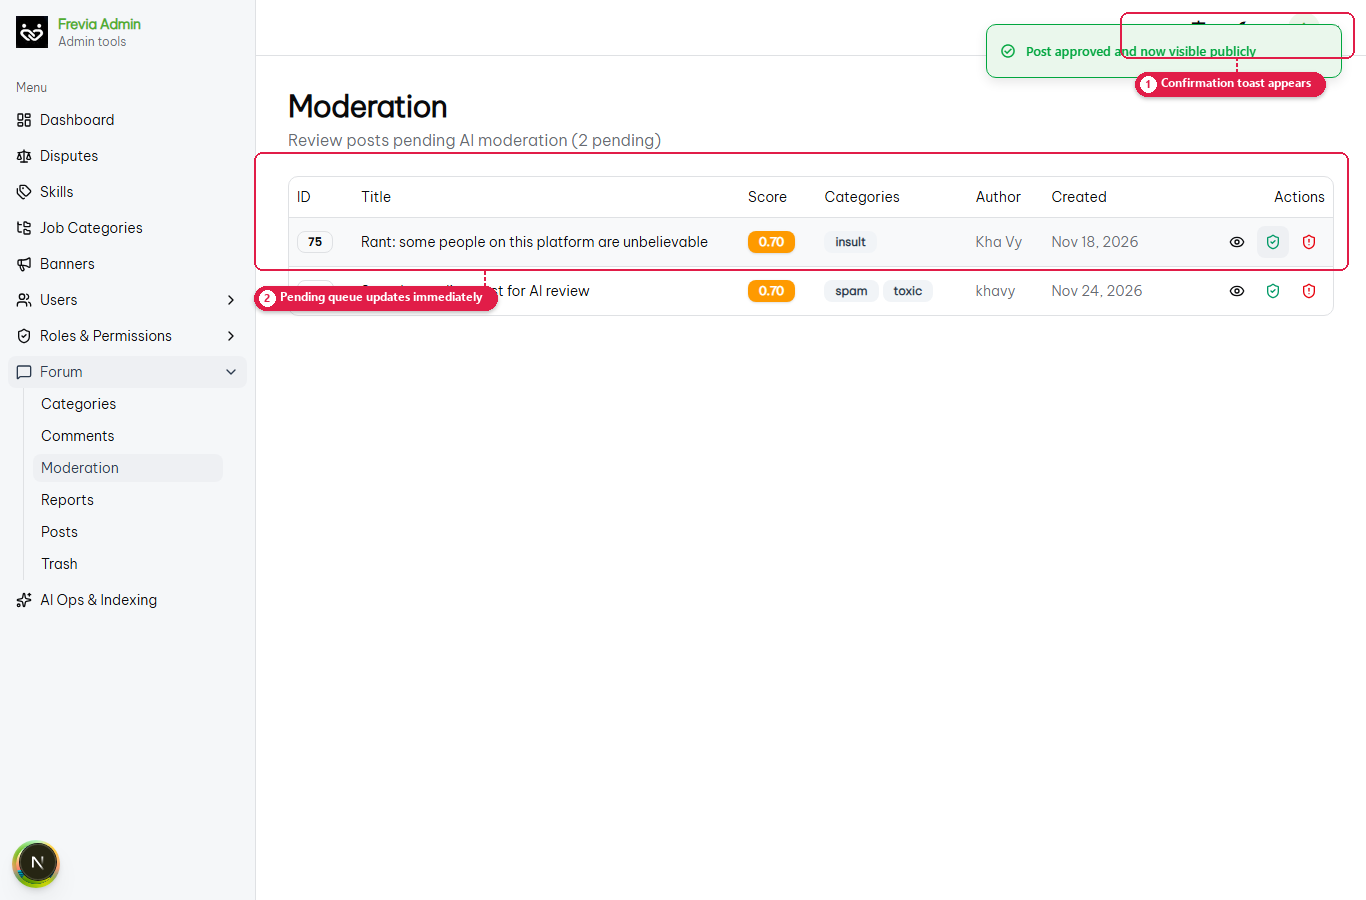
\includegraphics[width=0.90\textwidth]{images/admin/moderation/m34_03_guide.png}
  \caption{Approving or rejecting a moderation item}
\end{figure}
\Needspace{6\baselineskip}\paragraph{Step-by-Step User Guide:}
\begin{enumerate}[leftmargin=1.8em,itemsep=3pt]
  \item \rbadge{1} \textbf{Enter Resolution Notes:} Type optional reviewer notes explaining your moderation decision.
  \item \rbadge{2} \textbf{Approve or Reject:} Click \textbf{Approve} to publish to the forum or \textbf{Reject} to move to Trash.
\end{enumerate}
\Needspace{6\baselineskip}\paragraph{After You Submit (Result \& Troubleshooting):}
\begin{itemize}[leftmargin=1.5em,itemsep=2pt]
  \item \textbf{What Happens Next:} The item status updates immediately and logs the reviewing administrator.
  \item \textbf{Troubleshooting \& Common Messages:} Already-resolved items cannot be re-resolved.
\end{itemize}

\subsubsection{M35.01 -- View ID Verification Request List (UC-35.01)}
\begin{itemize}[leftmargin=1.5em,itemsep=2pt]
  \item \textbf{Screen Name \& Route Path:} ID Verification List -- \texttt{/admin/identity-verifications}.
  \item \textbf{Who Can Use This:} Administrator.
  \item \Needspace{6\baselineskip}\textbf{Before You Begin:} Signed in as Administrator.
\end{itemize}
\begin{figure}[H]\centering
  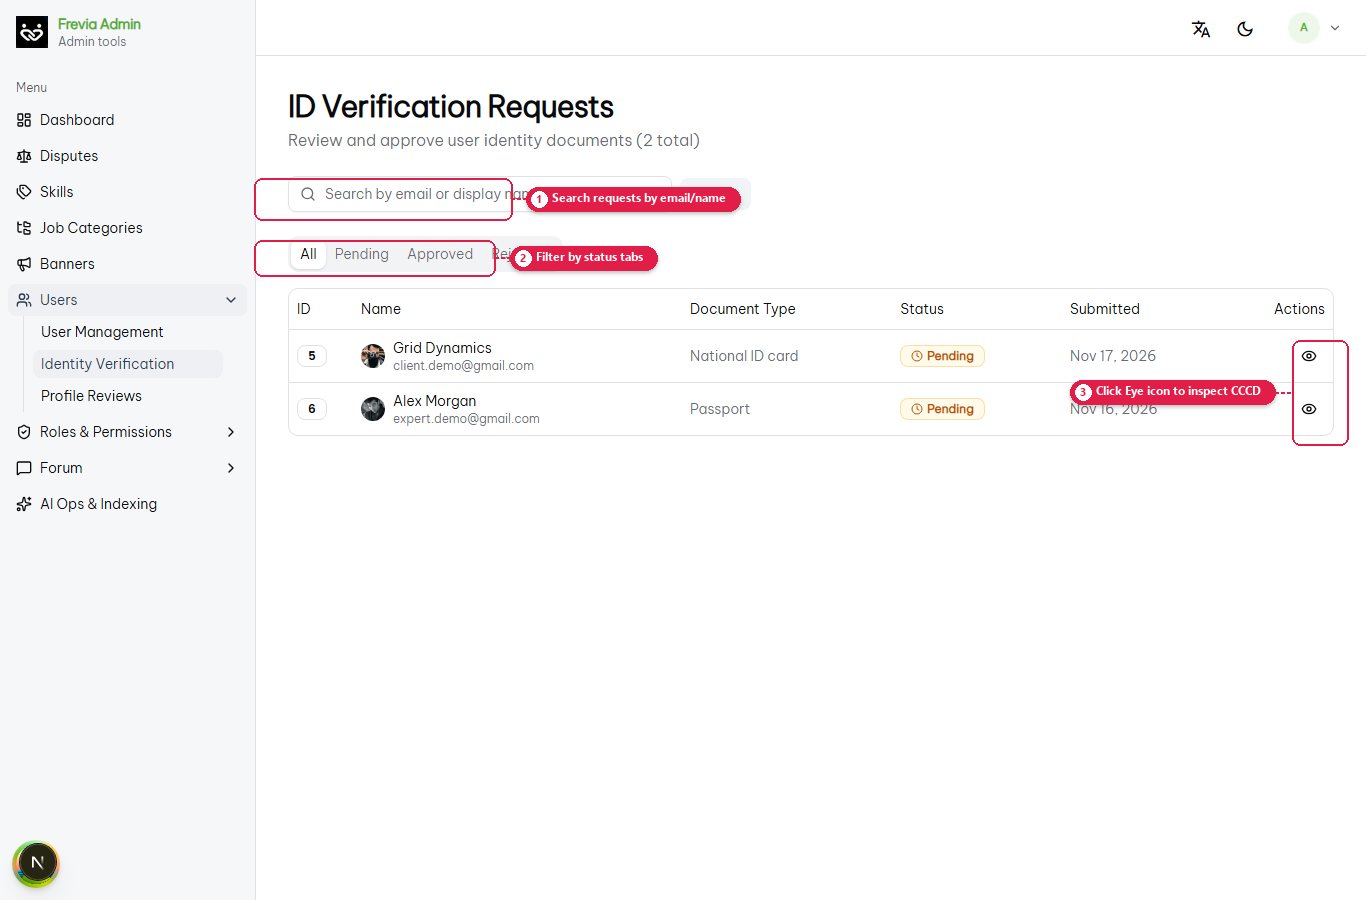
\includegraphics[width=0.90\textwidth]{images/admin/identity/m35_01_guide.png}
  \caption{Admin ID Verification Request queue}
\end{figure}
\Needspace{6\baselineskip}\paragraph{Step-by-Step User Guide:}
\begin{enumerate}[leftmargin=1.8em,itemsep=3pt]
  \item \rbadge{1} \textbf{Search \& Filter eKYC:} Filter verification requests by Pending, Approved, or Rejected status.
  \item \rbadge{2} \textbf{Review Table Summary:} Inspect applicant name, email, document type, and submission timestamp.
  \item \rbadge{3} \textbf{Open Request Detail:} Click the Eye icon to open the CCCD inspection modal.
\end{enumerate}
\Needspace{6\baselineskip}\paragraph{After You Submit (Result \& Troubleshooting):}
\begin{itemize}[leftmargin=1.5em,itemsep=2pt]
  \item \textbf{What Happens Next:} All user eKYC verification submissions are displayed in tabular order.
  \item \textbf{Troubleshooting \& Common Messages:} Empty queue shows a clean no-pending-requests state.
\end{itemize}

\subsubsection{M35.02 -- View ID Verification Request Detail (UC-35.02)}
\begin{itemize}[leftmargin=1.5em,itemsep=2pt]
  \item \textbf{Screen Name \& Route Path:} ID Verification Modal -- \texttt{/admin/identity-verifications}.
  \item \textbf{Who Can Use This:} Administrator.
  \item \Needspace{6\baselineskip}\textbf{Before You Begin:} Target verification request exists.
\end{itemize}
\begin{figure}[H]\centering
  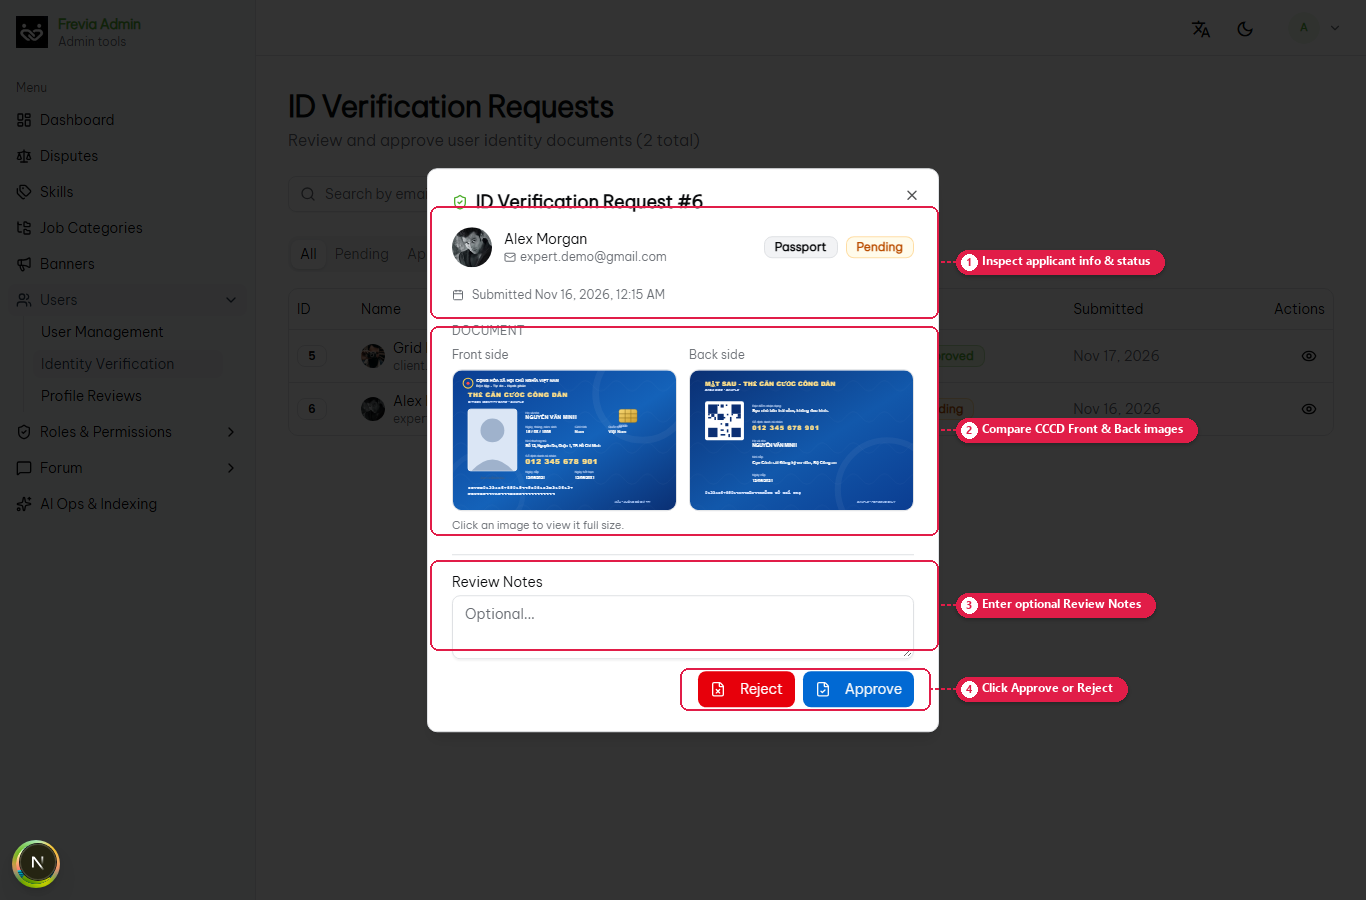
\includegraphics[width=0.90\textwidth]{images/admin/identity/m35_02_id_review_guide.png}
  \caption{Admin Reviewing CCCD Images and Verification Detail}
\end{figure}
\Needspace{6\baselineskip}\paragraph{Step-by-Step User Guide:}
\begin{enumerate}[leftmargin=1.8em,itemsep=3pt]
  \item \rbadge{1} \textbf{Inspect Applicant Info:} Verify applicant name, email, document type, and \texttt{Pending} badge.
  \item \rbadge{2} \textbf{Compare CCCD Images:} Inspect both uploaded CCCD Front and Back sides (click to zoom full-size).
  \item \rbadge{3} \textbf{Enter Review Notes:} Add optional review notes in the text box.
  \item \rbadge{4} \textbf{Choose Action:} Proceed to Approve or Reject based on document authenticity.
\end{enumerate}
\Needspace{6\baselineskip}\paragraph{After You Submit (Result \& Troubleshooting):}
\begin{itemize}[leftmargin=1.5em,itemsep=2pt]
  \item \textbf{What Happens Next:} Front/back CCCD images and extracted identity data are clearly displayed.
  \item \textbf{Troubleshooting \& Common Messages:} Corrupted image URLs display a fallback placeholder.
\end{itemize}

\subsubsection{M35.03 -- Approve ID Verification (UC-35.03)}
\begin{itemize}[leftmargin=1.5em,itemsep=2pt]
  \item \textbf{Screen Name \& Route Path:} ID Verification Modal -- \texttt{/admin/identity-verifications}.
  \item \textbf{Who Can Use This:} Administrator.
  \item \Needspace{6\baselineskip}\textbf{Before You Begin:} Request status is PENDING.
\end{itemize}
\begin{figure}[H]\centering
  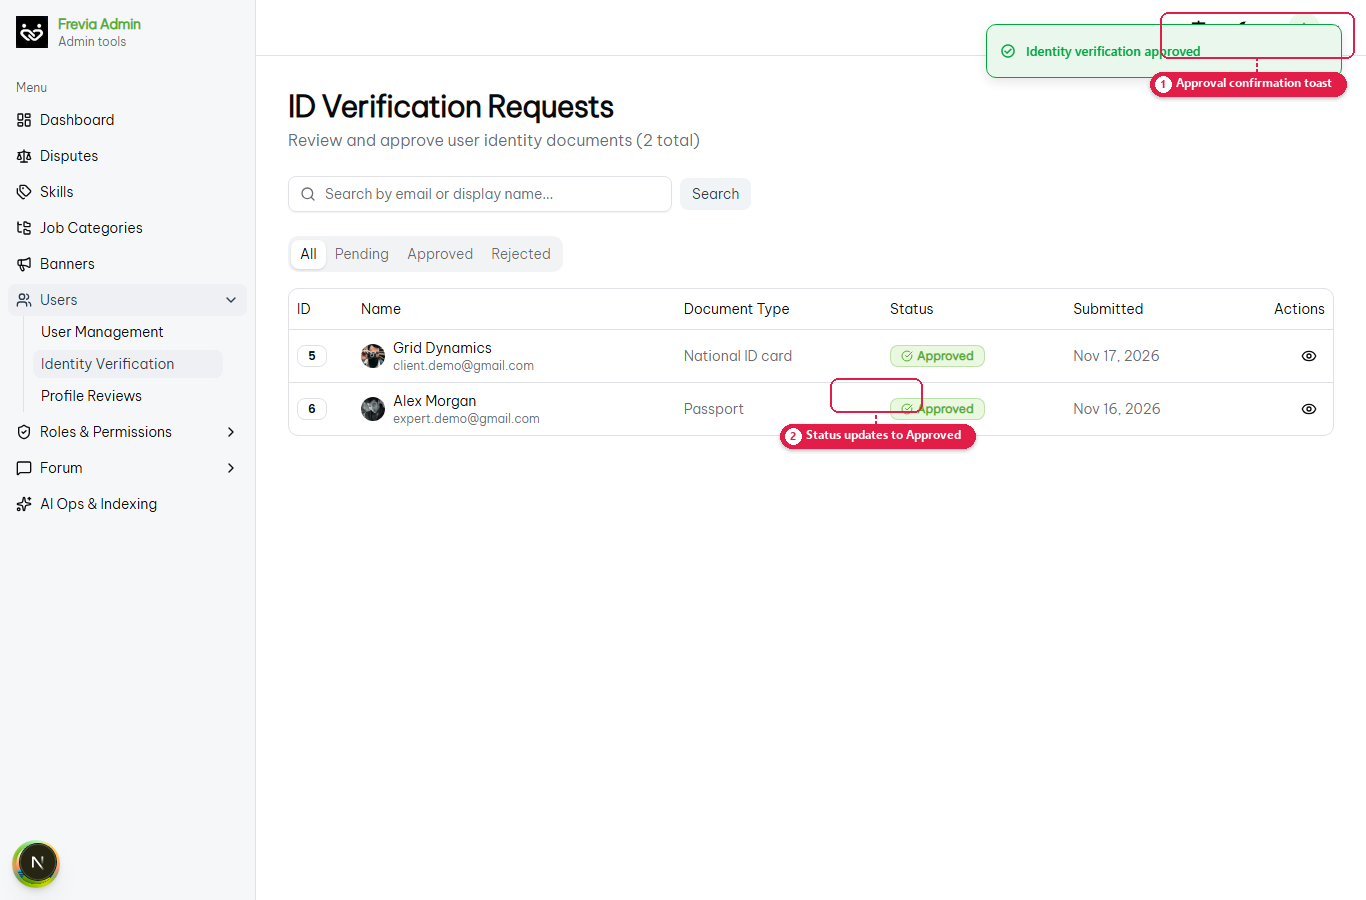
\includegraphics[width=0.90\textwidth]{images/admin/identity/m35_03_guide.png}
  \caption{Approving an eKYC identity verification request}
\end{figure}
\Needspace{6\baselineskip}\paragraph{Step-by-Step User Guide:}
\begin{enumerate}[leftmargin=1.8em,itemsep=3pt]
  \item \rbadge{1} \textbf{Add Approval Note:} Optionally enter internal verification notes.
  \item \rbadge{2} \textbf{Click Approve:} Click the blue \textbf{Approve} button to grant the user's Verified badge.
\end{enumerate}
\Needspace{6\baselineskip}\paragraph{After You Submit (Result \& Troubleshooting):}
\begin{itemize}[leftmargin=1.5em,itemsep=2pt]
  \item \textbf{What Happens Next:} Status changes to \texttt{APPROVED} and the user immediately receives the Verified Shield badge.
  \item \textbf{Troubleshooting \& Common Messages:} Duplicate approvals on already-approved requests are prevented.
\end{itemize}

\subsubsection{M35.04 -- Reject ID Verification (UC-35.04)}
\begin{itemize}[leftmargin=1.5em,itemsep=2pt]
  \item \textbf{Screen Name \& Route Path:} ID Verification Modal -- \texttt{/admin/identity-verifications}.
  \item \textbf{Who Can Use This:} Administrator.
  \item \Needspace{6\baselineskip}\textbf{Before You Begin:} Request status is PENDING.
\end{itemize}
\begin{figure}[H]\centering
  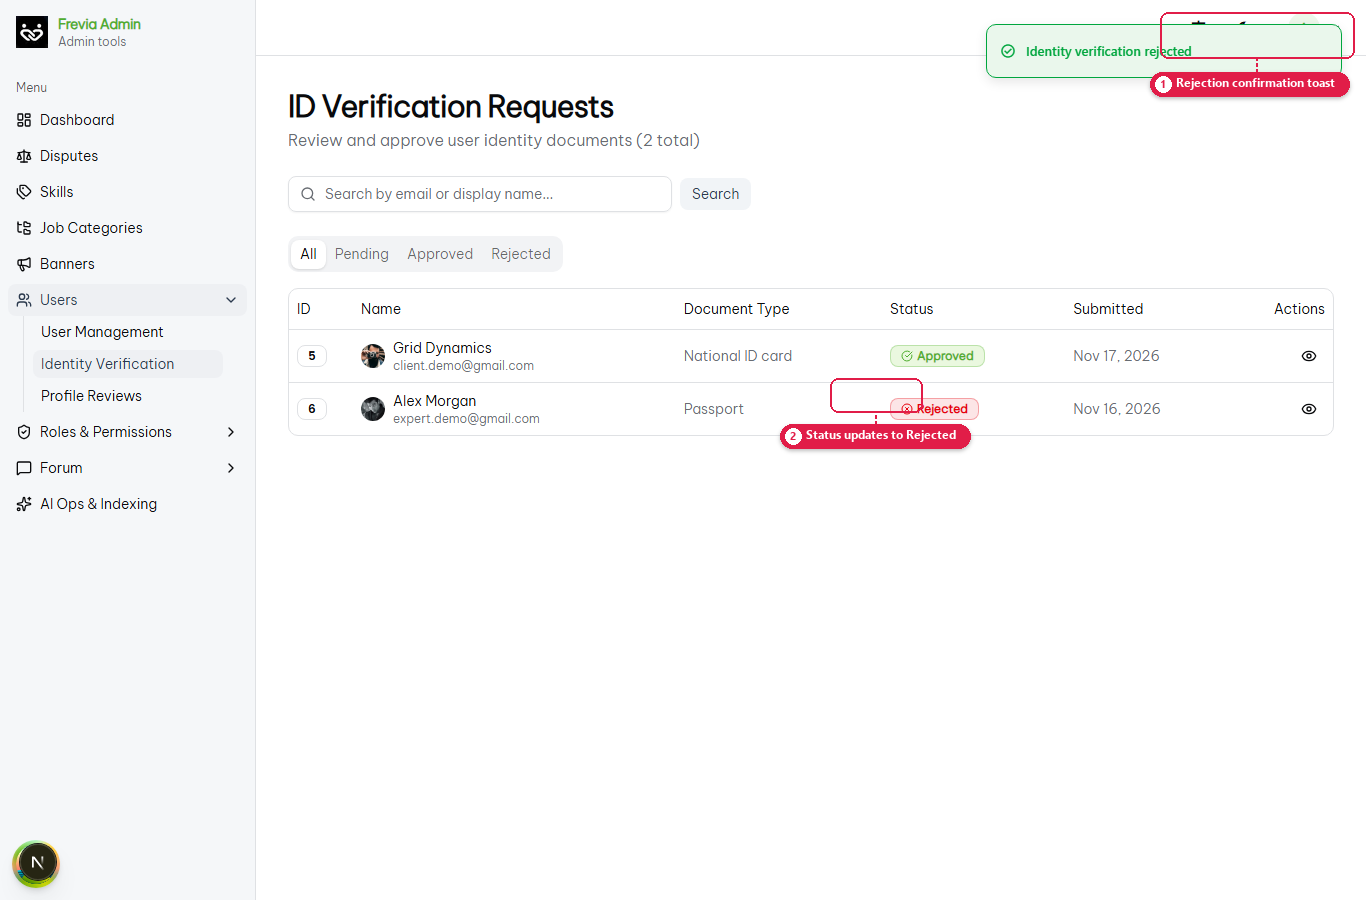
\includegraphics[width=0.90\textwidth]{images/admin/identity/m35_04_guide.png}
  \caption{Rejecting an eKYC verification request with reason}
\end{figure}
\Needspace{6\baselineskip}\paragraph{Step-by-Step User Guide:}
\begin{enumerate}[leftmargin=1.8em,itemsep=3pt]
  \item \rbadge{1} \textbf{Enter Rejection Reason:} Provide a clear explanation (e.g., blurry CCCD, face mismatch) in Review Notes.
  \item \rbadge{2} \textbf{Click Reject:} Click the red \textbf{Reject} button to decline the submission.
\end{enumerate}
\Needspace{6\baselineskip}\paragraph{After You Submit (Result \& Troubleshooting):}
\begin{itemize}[leftmargin=1.5em,itemsep=2pt]
  \item \textbf{What Happens Next:} Status updates to \texttt{REJECTED} and the user is notified to re-upload valid documents.
  \item \textbf{Troubleshooting \& Common Messages:} Rejection without a clear reason triggers a validation prompt.
\end{itemize}

\subsubsection{M36.01 -- View Deleted Posts/Comments List (UC-36.01)}
\begin{itemize}[leftmargin=1.5em,itemsep=2pt]
  \item \textbf{Screen Name \& Route Path:} Forum Trash -- \texttt{/admin/forum/trash}.
  \item \textbf{Who Can Use This:} Administrator.
  \item \Needspace{6\baselineskip}\textbf{Before You Begin:} Signed in as Administrator.
\end{itemize}
\begin{figure}[H]\centering
  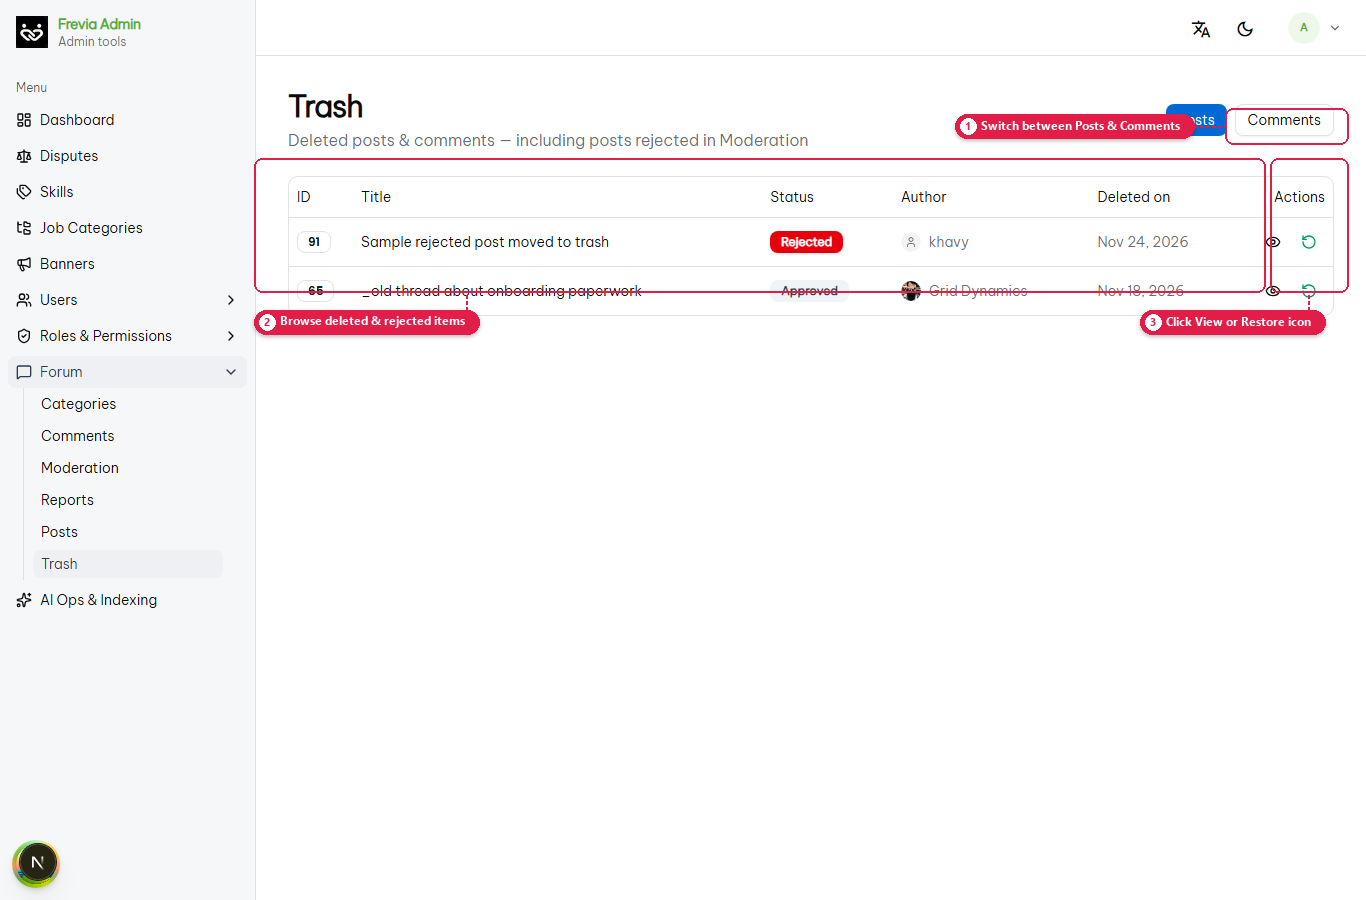
\includegraphics[width=0.90\textwidth]{images/admin/trash/m36_01_trash_guide.png}
  \caption{Admin Forum Trash list of soft-deleted and rejected items}
\end{figure}
\Needspace{6\baselineskip}\paragraph{Step-by-Step User Guide:}
\begin{enumerate}[leftmargin=1.8em,itemsep=3pt]
  \item \rbadge{1} \textbf{Switch Tabs:} Toggle between \textbf{Deleted Posts} and \textbf{Deleted Comments}.
  \item \rbadge{2} \textbf{Browse Archived Items:} Review soft-deleted or AI-rejected items along with deletion timestamps.
  \item \rbadge{3} \textbf{Restore Item:} Click the \textbf{Restore} icon next to an item to recover it.
\end{enumerate}
\Needspace{6\baselineskip}\paragraph{After You Submit (Result \& Troubleshooting):}
\begin{itemize}[leftmargin=1.5em,itemsep=2pt]
  \item \textbf{What Happens Next:} Paginated deleted and rejected forum items load cleanly.
  \item \textbf{Troubleshooting \& Common Messages:} If trash is empty, an empty-trash state is rendered.
\end{itemize}

\subsubsection{M36.02 -- View Deleted Posts/Comments Detail (UC-36.02)}
\begin{itemize}[leftmargin=1.5em,itemsep=2pt]
  \item \textbf{Screen Name \& Route Path:} Trash Detail Modal -- \texttt{/admin/forum/trash}.
  \item \textbf{Who Can Use This:} Administrator.
  \item \Needspace{6\baselineskip}\textbf{Before You Begin:} Deleted item exists in Forum Trash.
\end{itemize}
\begin{figure}[H]\centering
  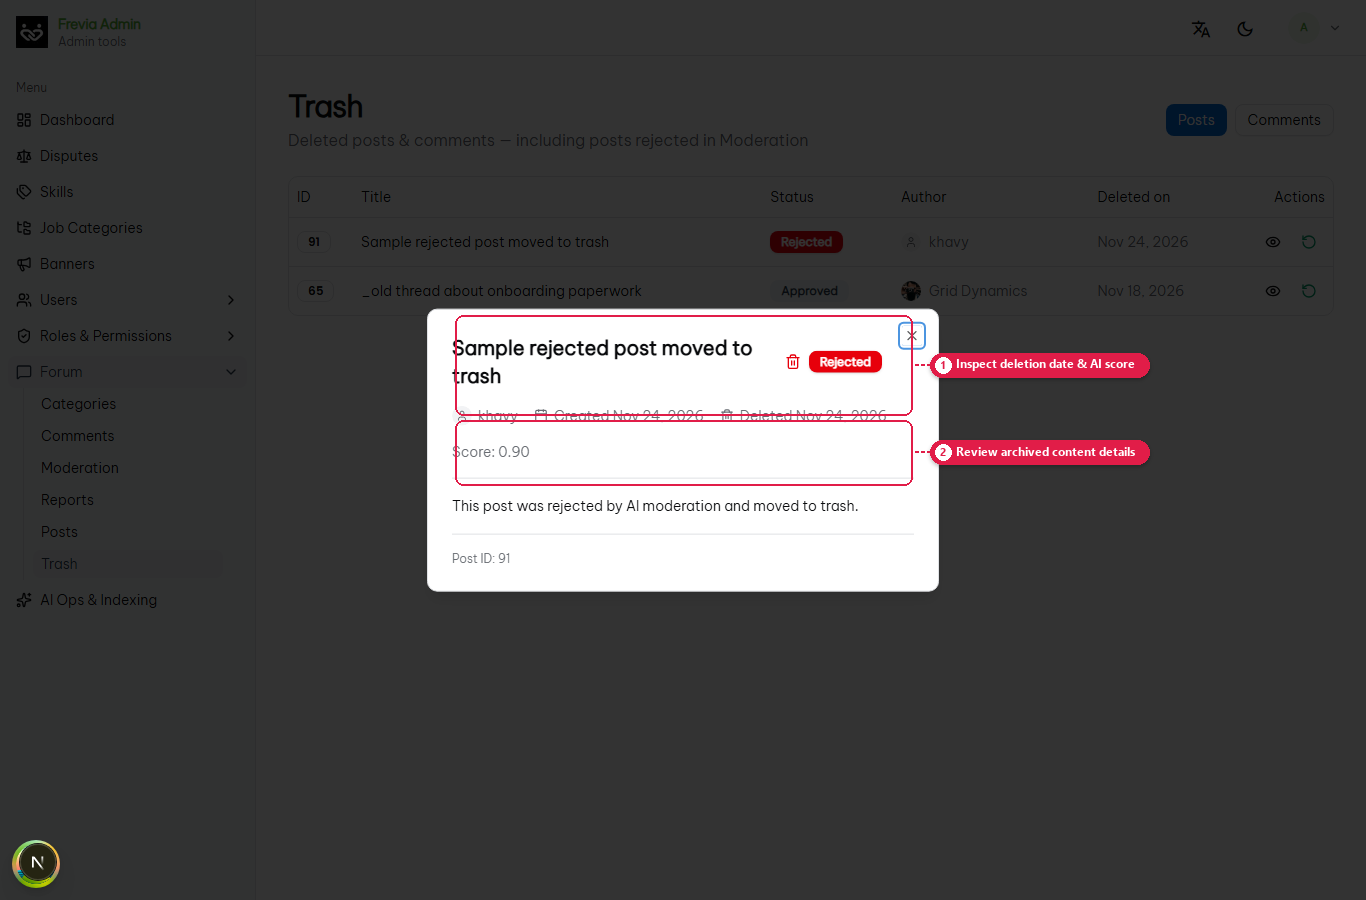
\includegraphics[width=0.90\textwidth]{images/admin/trash/m36_02_guide.png}
  \caption{Inspecting deleted or rejected forum item details}
\end{figure}
\Needspace{6\baselineskip}\paragraph{Step-by-Step User Guide:}
\begin{enumerate}[leftmargin=1.8em,itemsep=3pt]
  \item \rbadge{1} \textbf{Inspect Deletion Metadata:} Check author, moderation score, and exact \texttt{deletedAt} timestamp.
  \item \rbadge{2} \textbf{Review Content:} Read the full archived post or comment body before restoring.
\end{enumerate}
\Needspace{6\baselineskip}\paragraph{After You Submit (Result \& Troubleshooting):}
\begin{itemize}[leftmargin=1.5em,itemsep=2pt]
  \item \textbf{What Happens Next:} Full archived details are shown inside the inspection dialog.
  \item \textbf{Troubleshooting \& Common Messages:} Invalid item IDs display a not-found toast.
\end{itemize}

\subsubsection{M36.03 -- Restore Deleted Posts/Comments (UC-36.03)}
\begin{itemize}[leftmargin=1.5em,itemsep=2pt]
  \item \textbf{Screen Name \& Route Path:} Trash Restore -- \texttt{/admin/forum/trash}.
  \item \textbf{Who Can Use This:} Administrator.
  \item \Needspace{6\baselineskip}\textbf{Before You Begin:} Item is soft-deleted or REJECTED in trash.
\end{itemize}
\begin{figure}[H]\centering
  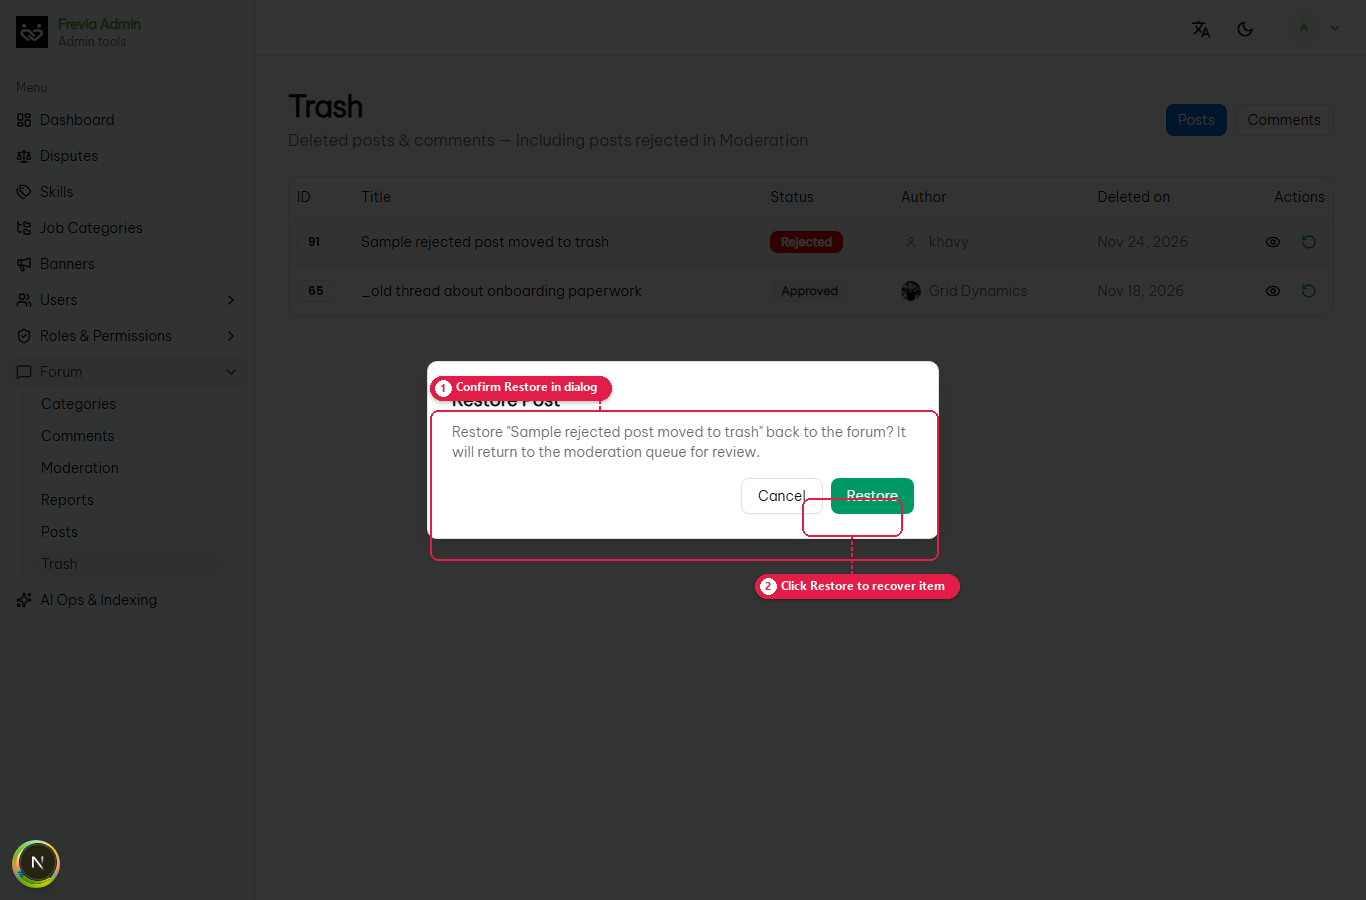
\includegraphics[width=0.90\textwidth]{images/admin/trash/m36_03_guide.png}
  \caption{Restoring a deleted or rejected forum item}
\end{figure}
\Needspace{6\baselineskip}\paragraph{Step-by-Step User Guide:}
\begin{enumerate}[leftmargin=1.8em,itemsep=3pt]
  \item \rbadge{1} \textbf{Click Restore:} Click the \textbf{Restore} button inside the trash list or detail modal.
\end{enumerate}
\Needspace{6\baselineskip}\paragraph{After You Submit (Result \& Troubleshooting):}
\begin{itemize}[leftmargin=1.5em,itemsep=2pt]
  \item \textbf{What Happens Next:} Soft-deleted items clear \texttt{deletedAt}; rejected posts reset to \texttt{PENDING} for re-review.
  \item \textbf{Troubleshooting \& Common Messages:} Active items already restored cannot be restored twice.
\end{itemize}

